\documentclass{standalone}

\usepackage[OT1]{fontenc}
\renewcommand*\familydefault{\sfdefault}
\usepackage{helvet,sfmath}
\usepackage{siunitx}

\usepackage{tikz}
\usetikzlibrary{arrows,calc,patterns}
\usepackage{tikz,tkz-euclide}


\begin{document}


\tikzset{every picture/.style={line width=0.75pt}} %set default line width to 0.75pt        

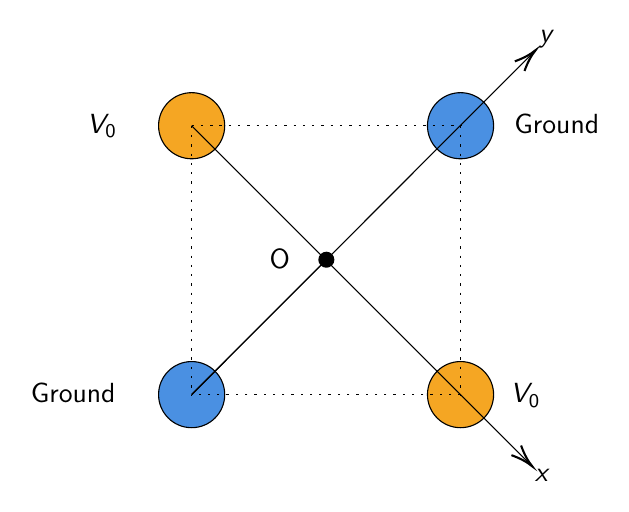
\begin{tikzpicture}[x=0.75pt,y=0.75pt,yscale=-1,xscale=1]
%uncomment if require: \path (0,721); %set diagram left start at 0, and has height of 721

%Shape: Circle [id:dp38493388739386125] 
\draw  [fill={rgb, 255:red, 245; green, 166; blue, 35 }  ,fill opacity=1 ] (477.79,451.95) .. controls (477.79,443.15) and (484.93,436.02) .. (493.73,436.02) .. controls (502.52,436.02) and (509.66,443.15) .. (509.66,451.95) .. controls (509.66,460.75) and (502.52,467.88) .. (493.73,467.88) .. controls (484.93,467.88) and (477.79,460.75) .. (477.79,451.95) -- cycle ;
%Shape: Ellipse [id:dp788887770241431] 
\draw  [fill={rgb, 255:red, 74; green, 144; blue, 226 }  ,fill opacity=1 ] (477.79,581.5) .. controls (477.79,572.71) and (484.93,565.57) .. (493.73,565.57) .. controls (502.52,565.57) and (509.66,572.71) .. (509.66,581.5) .. controls (509.66,590.3) and (502.52,597.44) .. (493.73,597.44) .. controls (484.93,597.44) and (477.79,590.3) .. (477.79,581.5) -- cycle ;
%Straight Lines [id:da9387645966454564] 
\draw  [dash pattern={on 0.84pt off 2.51pt}]  (493.73,451.95) -- (493.73,581.5) ;
%Shape: Circle [id:dp9951636459340562] 
\draw  [fill={rgb, 255:red, 74; green, 144; blue, 226 }  ,fill opacity=1 ] (607.35,451.95) .. controls (607.35,443.15) and (614.48,436.02) .. (623.28,436.02) .. controls (632.08,436.02) and (639.21,443.15) .. (639.21,451.95) .. controls (639.21,460.75) and (632.08,467.88) .. (623.28,467.88) .. controls (614.48,467.88) and (607.35,460.75) .. (607.35,451.95) -- cycle ;
%Shape: Ellipse [id:dp4760811520051388] 
\draw  [fill={rgb, 255:red, 245; green, 166; blue, 35 }  ,fill opacity=1 ] (607.35,581.5) .. controls (607.35,572.71) and (614.48,565.57) .. (623.28,565.57) .. controls (632.08,565.57) and (639.21,572.71) .. (639.21,581.5) .. controls (639.21,590.3) and (632.08,597.44) .. (623.28,597.44) .. controls (614.48,597.44) and (607.35,590.3) .. (607.35,581.5) -- cycle ;
%Straight Lines [id:da1925782064441528] 
\draw    (493.73,451.95) -- (656.44,614.67) ;
\draw [shift={(657.86,616.08)}, rotate = 225] [color={rgb, 255:red, 0; green, 0; blue, 0 }  ][line width=0.75]    (10.93,-3.29) .. controls (6.95,-1.4) and (3.31,-0.3) .. (0,0) .. controls (3.31,0.3) and (6.95,1.4) .. (10.93,3.29)   ;
%Straight Lines [id:da7409281123995733] 
\draw    (493.73,581.5) -- (658.09,416.92) ;
\draw [shift={(659.5,415.5)}, rotate = 134.96] [color={rgb, 255:red, 0; green, 0; blue, 0 }  ][line width=0.75]    (10.93,-3.29) .. controls (6.95,-1.4) and (3.31,-0.3) .. (0,0) .. controls (3.31,0.3) and (6.95,1.4) .. (10.93,3.29)   ;
%Straight Lines [id:da37729956897385686] 
\draw    (493.73,581.5) -- (558.63,516.51) ;
\draw [shift={(558.63,516.51)}, rotate = 314.96] [color={rgb, 255:red, 0; green, 0; blue, 0 }  ][fill={rgb, 255:red, 0; green, 0; blue, 0 }  ][line width=0.75]      (0, 0) circle [x radius= 3.35, y radius= 3.35]   ;
%Straight Lines [id:da6340048690425479] 
\draw  [dash pattern={on 0.84pt off 2.51pt}]  (623.28,451.95) -- (623.28,581.5) ;
%Straight Lines [id:da8082558315415289] 
\draw  [dash pattern={on 0.84pt off 2.51pt}]  (623.28,581.5) -- (493.73,581.5) ;
%Straight Lines [id:da09105101079858435] 
\draw  [dash pattern={on 0.84pt off 2.51pt}]  (493.73,451.95) -- (623.28,451.95) ;

% Text Node
\draw (415,575) node [anchor=north west][inner sep=0.75pt]   [align=left] {Ground};
% Text Node
\draw (648,445) node [anchor=north west][inner sep=0.75pt]   [align=left] {Ground};
% Text Node
\draw (657.86,616.08) node [anchor=north west][inner sep=0.75pt]    {$x$};
% Text Node
\draw (659.86,415.5) node [anchor=south west] [inner sep=0.75pt]    {$y$};
% Text Node
\draw (646,575) node [anchor=north west][inner sep=0.75pt]    {$V_{0}$};
% Text Node
\draw (442,445) node [anchor=north west][inner sep=0.75pt]    {$V_{0}$};
% Text Node
\draw (530,510) node [anchor=north west][inner sep=0.75pt]   [align=left] {O};


\end{tikzpicture}



\end{document}